\section{FLASH-RT}

    %%%%%%%%%%%%%%%%%%%%%%%%%%%%%%%%%%%%%%%%
    %%  Slide 1: <>  %%
    %%%%%%%%%%%%%%%%%%%%%%%%%%%%%%%%%%%%%%%%
    \begin{frame}
        \frametitle{FLASH radiotherapy}
        \begin{itemize}
            \item Radiotherapy takes advantage of the damage causes by the ionization of energy loss by particles
            \item FLASH-RT consists in delivering a high level of dose in a small fraction of time: this seems reducing the toxiticy of the radiation on healty tissues
            \item FLASH-RT and the medical applicability are still \textbf{under test}!
        \end{itemize}
        \medskip
        \begin{columns}
            \column{0.5\textwidth}  
                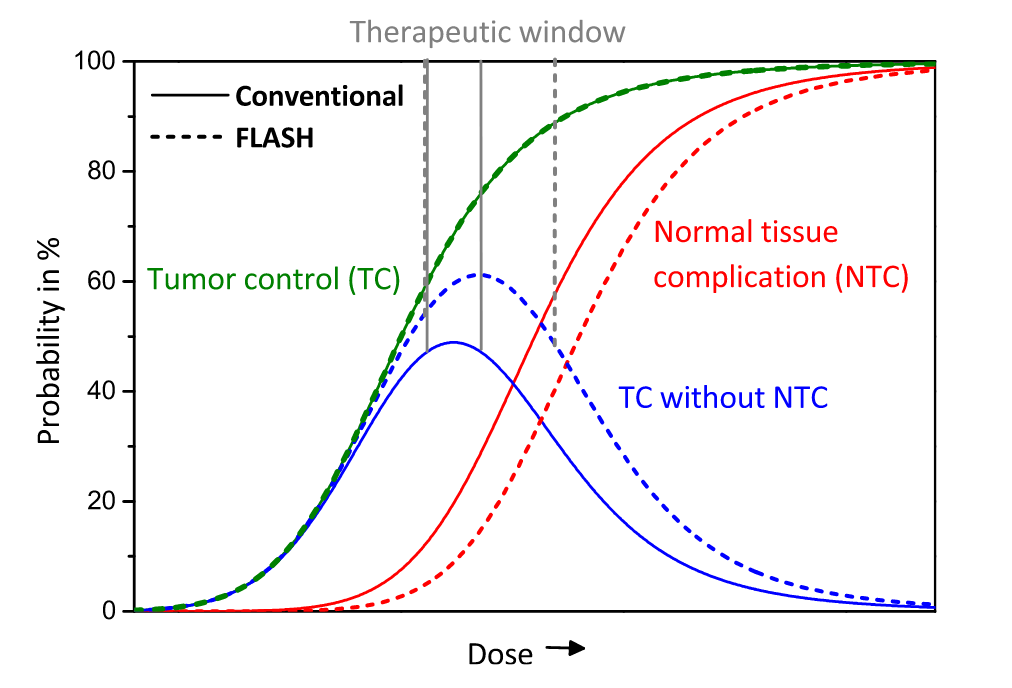
\includegraphics[width=1.2\linewidth]{figures/pixel_detectors_usage/curve_flash.png}
        \column{0.5\textwidth} 
            \begin{itemize}
                \item %FLASH-RT is still \textbf{under test}!
                \begin{itemize}
                    \item medical aspect: in vitro and with animals; only one patient has been treated
                    \item  bio-physics aspect: dependence of the FLASH effect on the treatment conditions 
                    \item  strumental aspect: need for new detectors
                \end{itemize}
            \end{itemize}
        \end{columns}
    \end{frame} 


    %%%%%%%%%%%%%%%%%%%%%%%%%%%%%%%%%%%%%%%%
    %%  Slide 1: <>  %%
    %%%%%%%%%%%%%%%%%%%%%%%%%%%%%%%%%%%%%%%%
    \begin{frame}
        \frametitle{Electron FLASH-RT}
        QUESTA È DA CAPIRE COME MODELLARLA! 
        \centering
        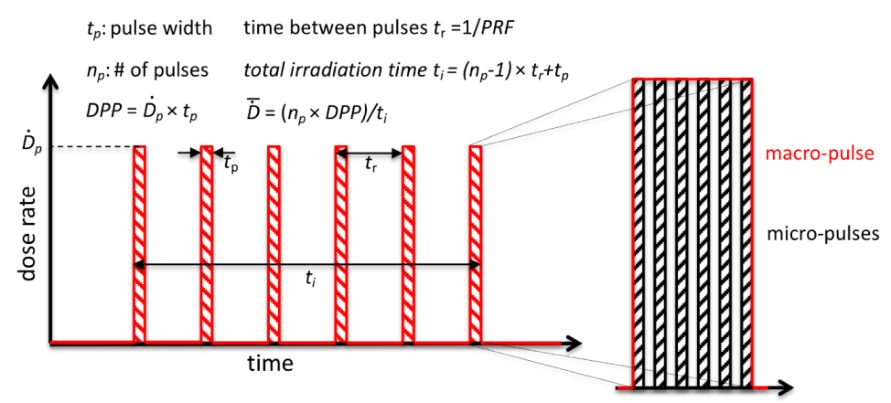
\includegraphics[width=0.8\linewidth]{figures/test_beam/beam_structure.pdf}
        \begin{columns}
            \column{0.5\textwidth}  
                \begin{table}
                    \tiny
                    \begin{center}
                    \begin{tabular}{|c | c |c |}
                    \hline
                    & CONV-RT & FLASH-RT \\
                    \hline
                    \hline
                    Dose rate & \SI{0.03}{Gy/s} & \SI{40}{Gy/s}\\
                    Intra pulse dose rate & \SI{100}{Gy/s}&\SI{10 6}{Gy/s}\\
                    Treatment duration & $\sim$minutes & $\lessapprox$\SI{500}{ms} \\
                    Dose Per Pulse & \SI{0.3}{mGy} & 1-10 Gy\\
                    Pulse width & \SI{3}{\us} & $\sim$\SI{2}{\us} \\
                    \hline
                    \end{tabular}
                    \end{center}
                \end{table}    
            \column{0.55\textwidth}
                \begin{equation*}
                    N_A[/\si{\cm\squared}] = \frac{DPP[Gy]}{10^{10} S[\si{MeV \cm \squared /g}]}
                \end{equation*}
        \end{columns}
        $N_A$ = 2.9 10$^9$/cm, F = 1.45$\times$10$^{10}$\si{MHz/cm\squared} @  DPP=\SI{1}{Gy}, t$_p$=\SI{2}{\us}
    \end{frame}     


    %%%%%%%%%%%%%%%%%%%%%%%%%%%%%%%%%%%%%%%%
    %%  Slide 1: <dosimeters>  %%
    %%%%%%%%%%%%%%%%%%%%%%%%%%%%%%%%%%%%%%%%
    \begin{frame}
        \frametitle{FLASH-RT: need for detectors}
        All online detectors show saturation problems at such high intensity
        \medskip
        \begin{columns}
            \column{0.4\textwidth} 
            Different types of detector with different charateristics are required: 
                \begin{itemize}
                    \item \textbf{dosimeters} 
                    \item \textbf{beam monitor} 
                    \item diagnostic 
                \end{itemize}
            \column{0.6\textwidth}  
                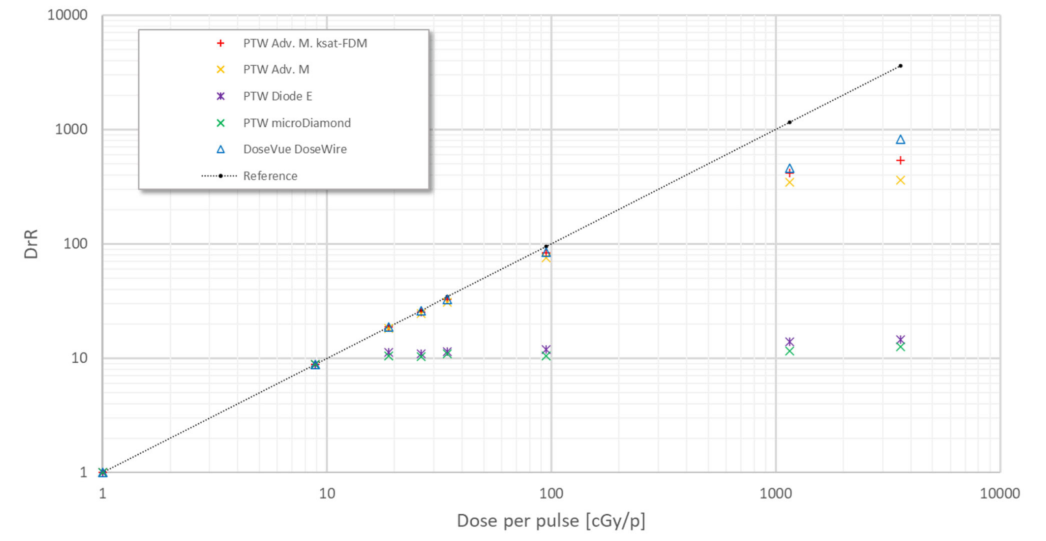
\includegraphics[width=1.1\linewidth]{figures/pixel_detectors_usage/saturation_dosimeters.pdf}
                %COSA SONO I COLORI
        \end{columns}
        \bigskip
        The applicability of MAPS \textbf{would} take advantage of: 
        \begin{enumerate}
            \item the small C$_D \sim$\si{fF} to have fast readout and discharge, which guaranties a rate capability of \SI{100}{MHz/cm\squared}, to split the DPP in many buckets and reduce the saturation effect
            \item the thinness $\sim$\SI{50}{\um} to have a costant high $E$ to prevent recombination and integrate the signal from many particles
        \end{enumerate}
    \end{frame}     


    %%%%%%%%%%%%%%%%%%%%%%%%%%%%%%%%%%%%
    %% Slide 2: <> %%
    %%%%%%%%%%%%%%%%%%%%%%%%%%%%%%%%%%%%
    \begin{frame}
        \frametitle{Test on the beam: ElectronFLASH}
        ElectronFLASH is the new accelerator for research on FLASH-RT placed in S. Chiara hospital in Pisa \\
        \medskip
        Accelerator charateristics: 
        \begin{itemize}
            \item linear accelerator
            \item bunched beam
            \item two energiy configurations 7-9\si{MeV}
            \item can reach ultra high intensity (over \SI{5000}{Gy/s})
            \item beam parameters can be configured independently from each other
            \item equipped with a set of plexiglass applicators (diameters in range from \SI{1}{cm} to \SI{12}{cm}) which are used to produce a uniform dose profile 
        \end{itemize}
    \end{frame}  

    %%%%%%%%%%%%%%%%%%%%%%%%%%%%%%%%%%%%
    %% Slide 2: <> %%
    %%%%%%%%%%%%%%%%%%%%%%%%%%%%%%%%%%%%
    \begin{frame}
        \frametitle{Test on the beam: experimental set up}
        In order to shield and protect the DUT and the electronics from the high fluence, 2 \textbf{collimators} and a \textbf{box} have been used. 
        \smallskip
        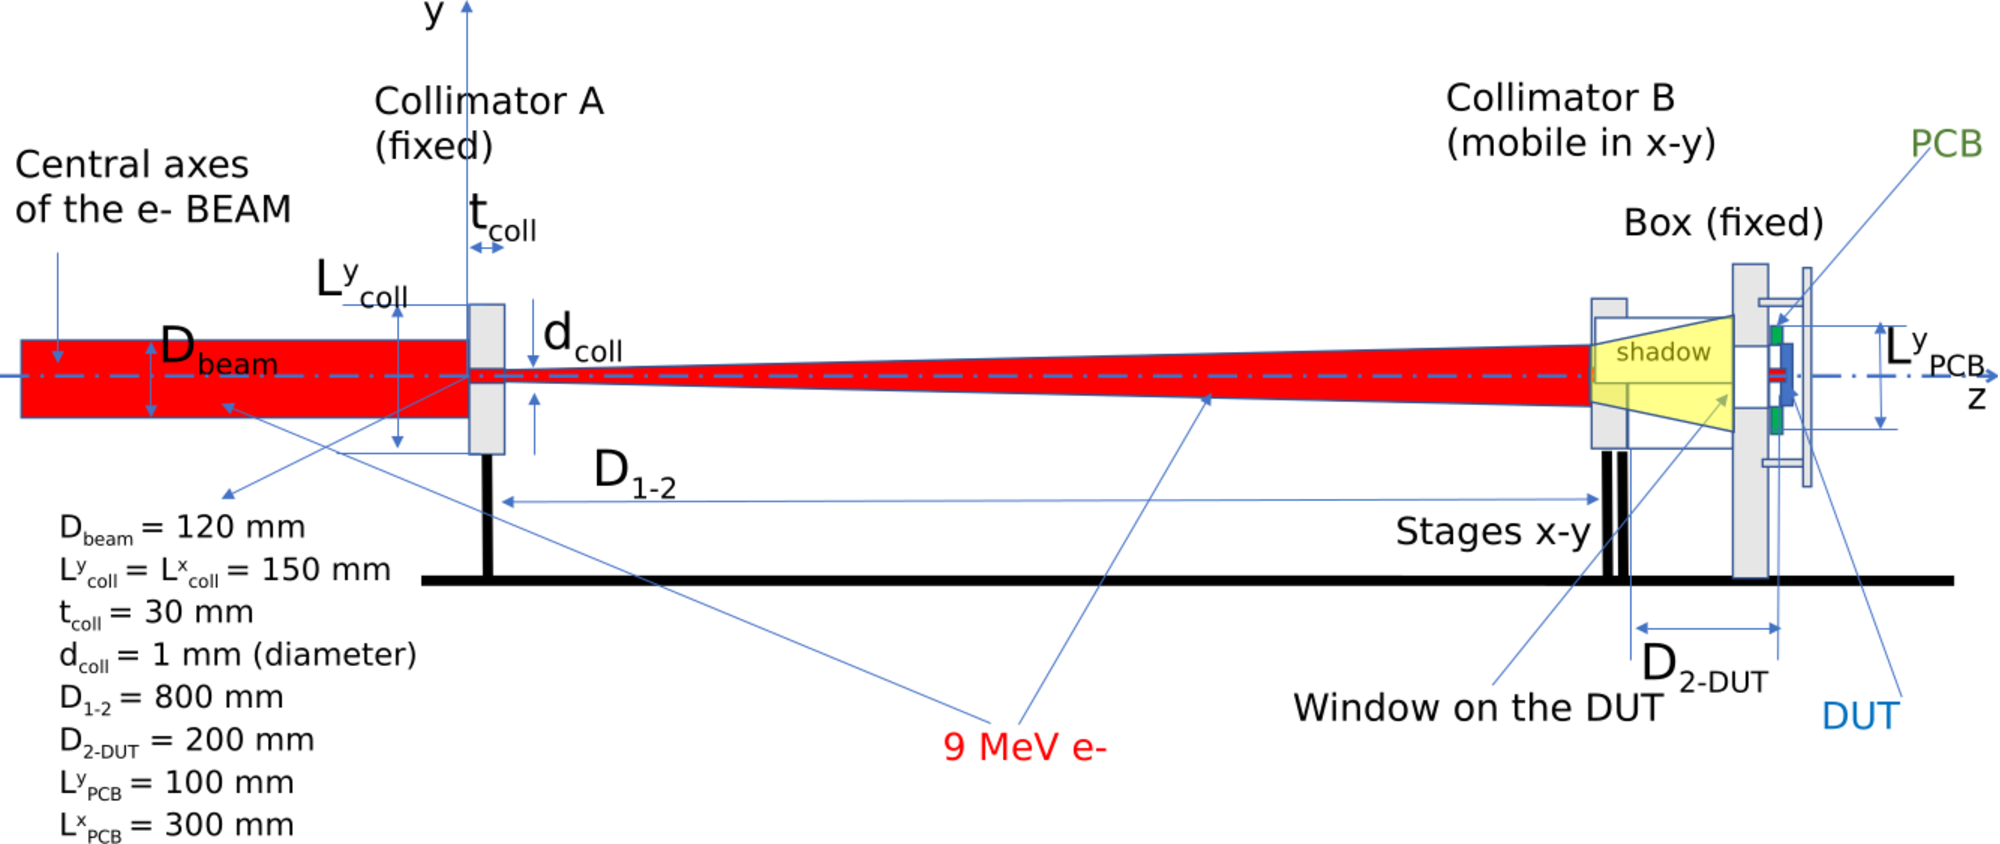
\includegraphics[width=.95\linewidth]{figures/test_beam/Flash-beam-scheme.pdf}\\
        \smallskip
        Coll. A is expected to dreacrease the fluence on the DUT of \textbf{4 10$^{-4}$}\\
        \medskip
        $N_A$ = 2.9 10$^9$/cm, F = 7.25$\times$10$^{9}$\si{MHz/cm\squared} @  DPP=\SI{1}{Gy}, t$_p$=\SI{4}{\us}
        
    \end{frame}    


    %%%%%%%%%%%%%%%%%%%%%%%%%%%%%%%%%%%%
    %% Slide 2: <> %%
    %%%%%%%%%%%%%%%%%%%%%%%%%%%%%%%%%%%%
    \begin{frame}
        \frametitle{Test on the beam: experimental set up}
        \centering
        \includegraphics[width=.7\linewidth]{figures/test_beam/testbeam_photos.pdf}  
    \end{frame}    


    %%%%%%%%%%%%%%%%%%%%%%%%%%%%%%%%%%%%
    %% Slide 2: <> %%
    %%%%%%%%%%%%%%%%%%%%%%%%%%%%%%%%%%%%
    \begin{frame}
        \frametitle{Test on the beam: preliminary results}
        \begin{columns}
            \column{0.5\textwidth} 
                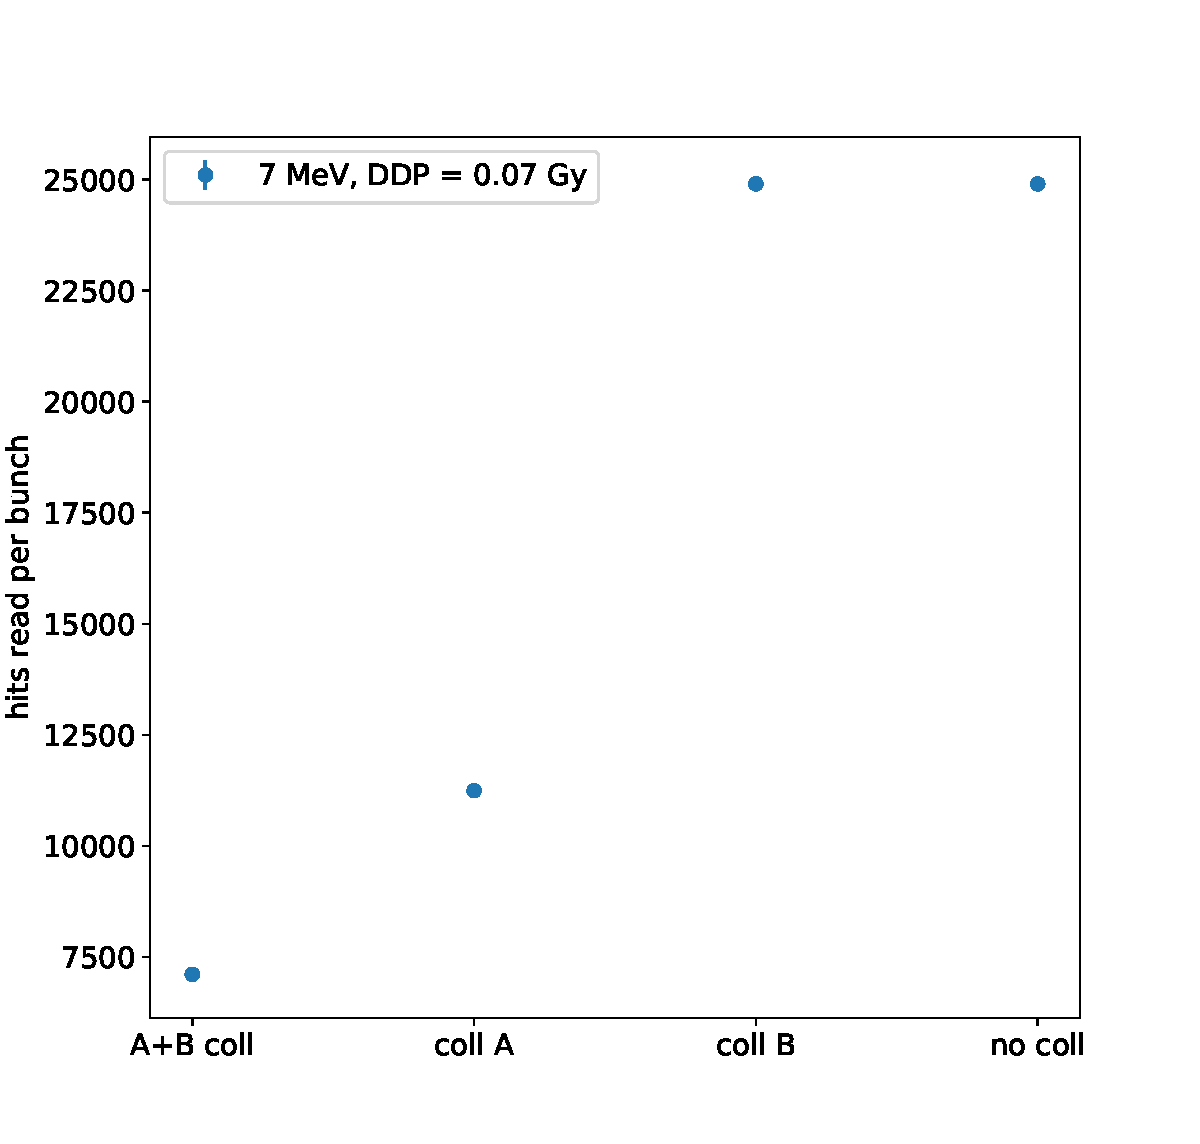
\includegraphics[width=1.1\linewidth]{figures/test_beam/hits.pdf}  
            \column{0.5\textwidth} 
                \begin{itemize}
                    \item under-extimation of the Bremsstrahlung production of electrons which stop in the collimators 
                    \item high background in data
                    \item saturation due to the readout system occurs without collimators
                    \item readout logic has been tested with high hit rate
                    \item need for a simulation to better understand the data
                \end{itemize}
            \end{columns}
        \end{frame}  